\begin{frame}
 \frametitle{Lembretes}
 \begin{enumerate}
  \item Sprints documentadas
  \item Releases - colocar na aba do github (olha owla)
  \item Organizar github com histórias, tasks, sprints (milestones) - transparência
  \item Em produção - (transparência) - entregas contínuas (por sprint)
  \item Post-mortem - continuamento registrado (retrospectivas)
  \item wiki - up-to-date
 \end{enumerate}
\end{frame}

\section{Contexto}
\begin{frame}
 \frametitle{Manifesto Ágil}
 \begin{enumerate}
  \item \textbf{Indivíduos e interação entre eles} mais que processos e ferramentas
  \item \textbf{Software em funcionamento}  mais que documentação abrangente
  \item \textbf{Colaboração com o cliente} mais que negociação de contratos
  \item \textbf{Responder a mudanças} mais que seguir um plano
 \end{enumerate}
\end{frame}

\begin{frame}
 \frametitle{Solução 1: Scrum}
 \begin{itemize}
  \item O framework Scrum consiste nos times do Scrum associadas a papéis, eventos, artefatos e
regras 	
  \item As regras do Scrum integram os eventos, papéis e artefatos, administrando as relações e
interações entre eles
 \end{itemize}
  \begin{block}{}
 Não há eventos, artefatos, boas práticas que focam na entrega de produto de qualidade
 \end{block}
\end{frame}

\begin{frame}
 \frametitle{Scrum - Framework}
  \begin{figure}
   \centering
   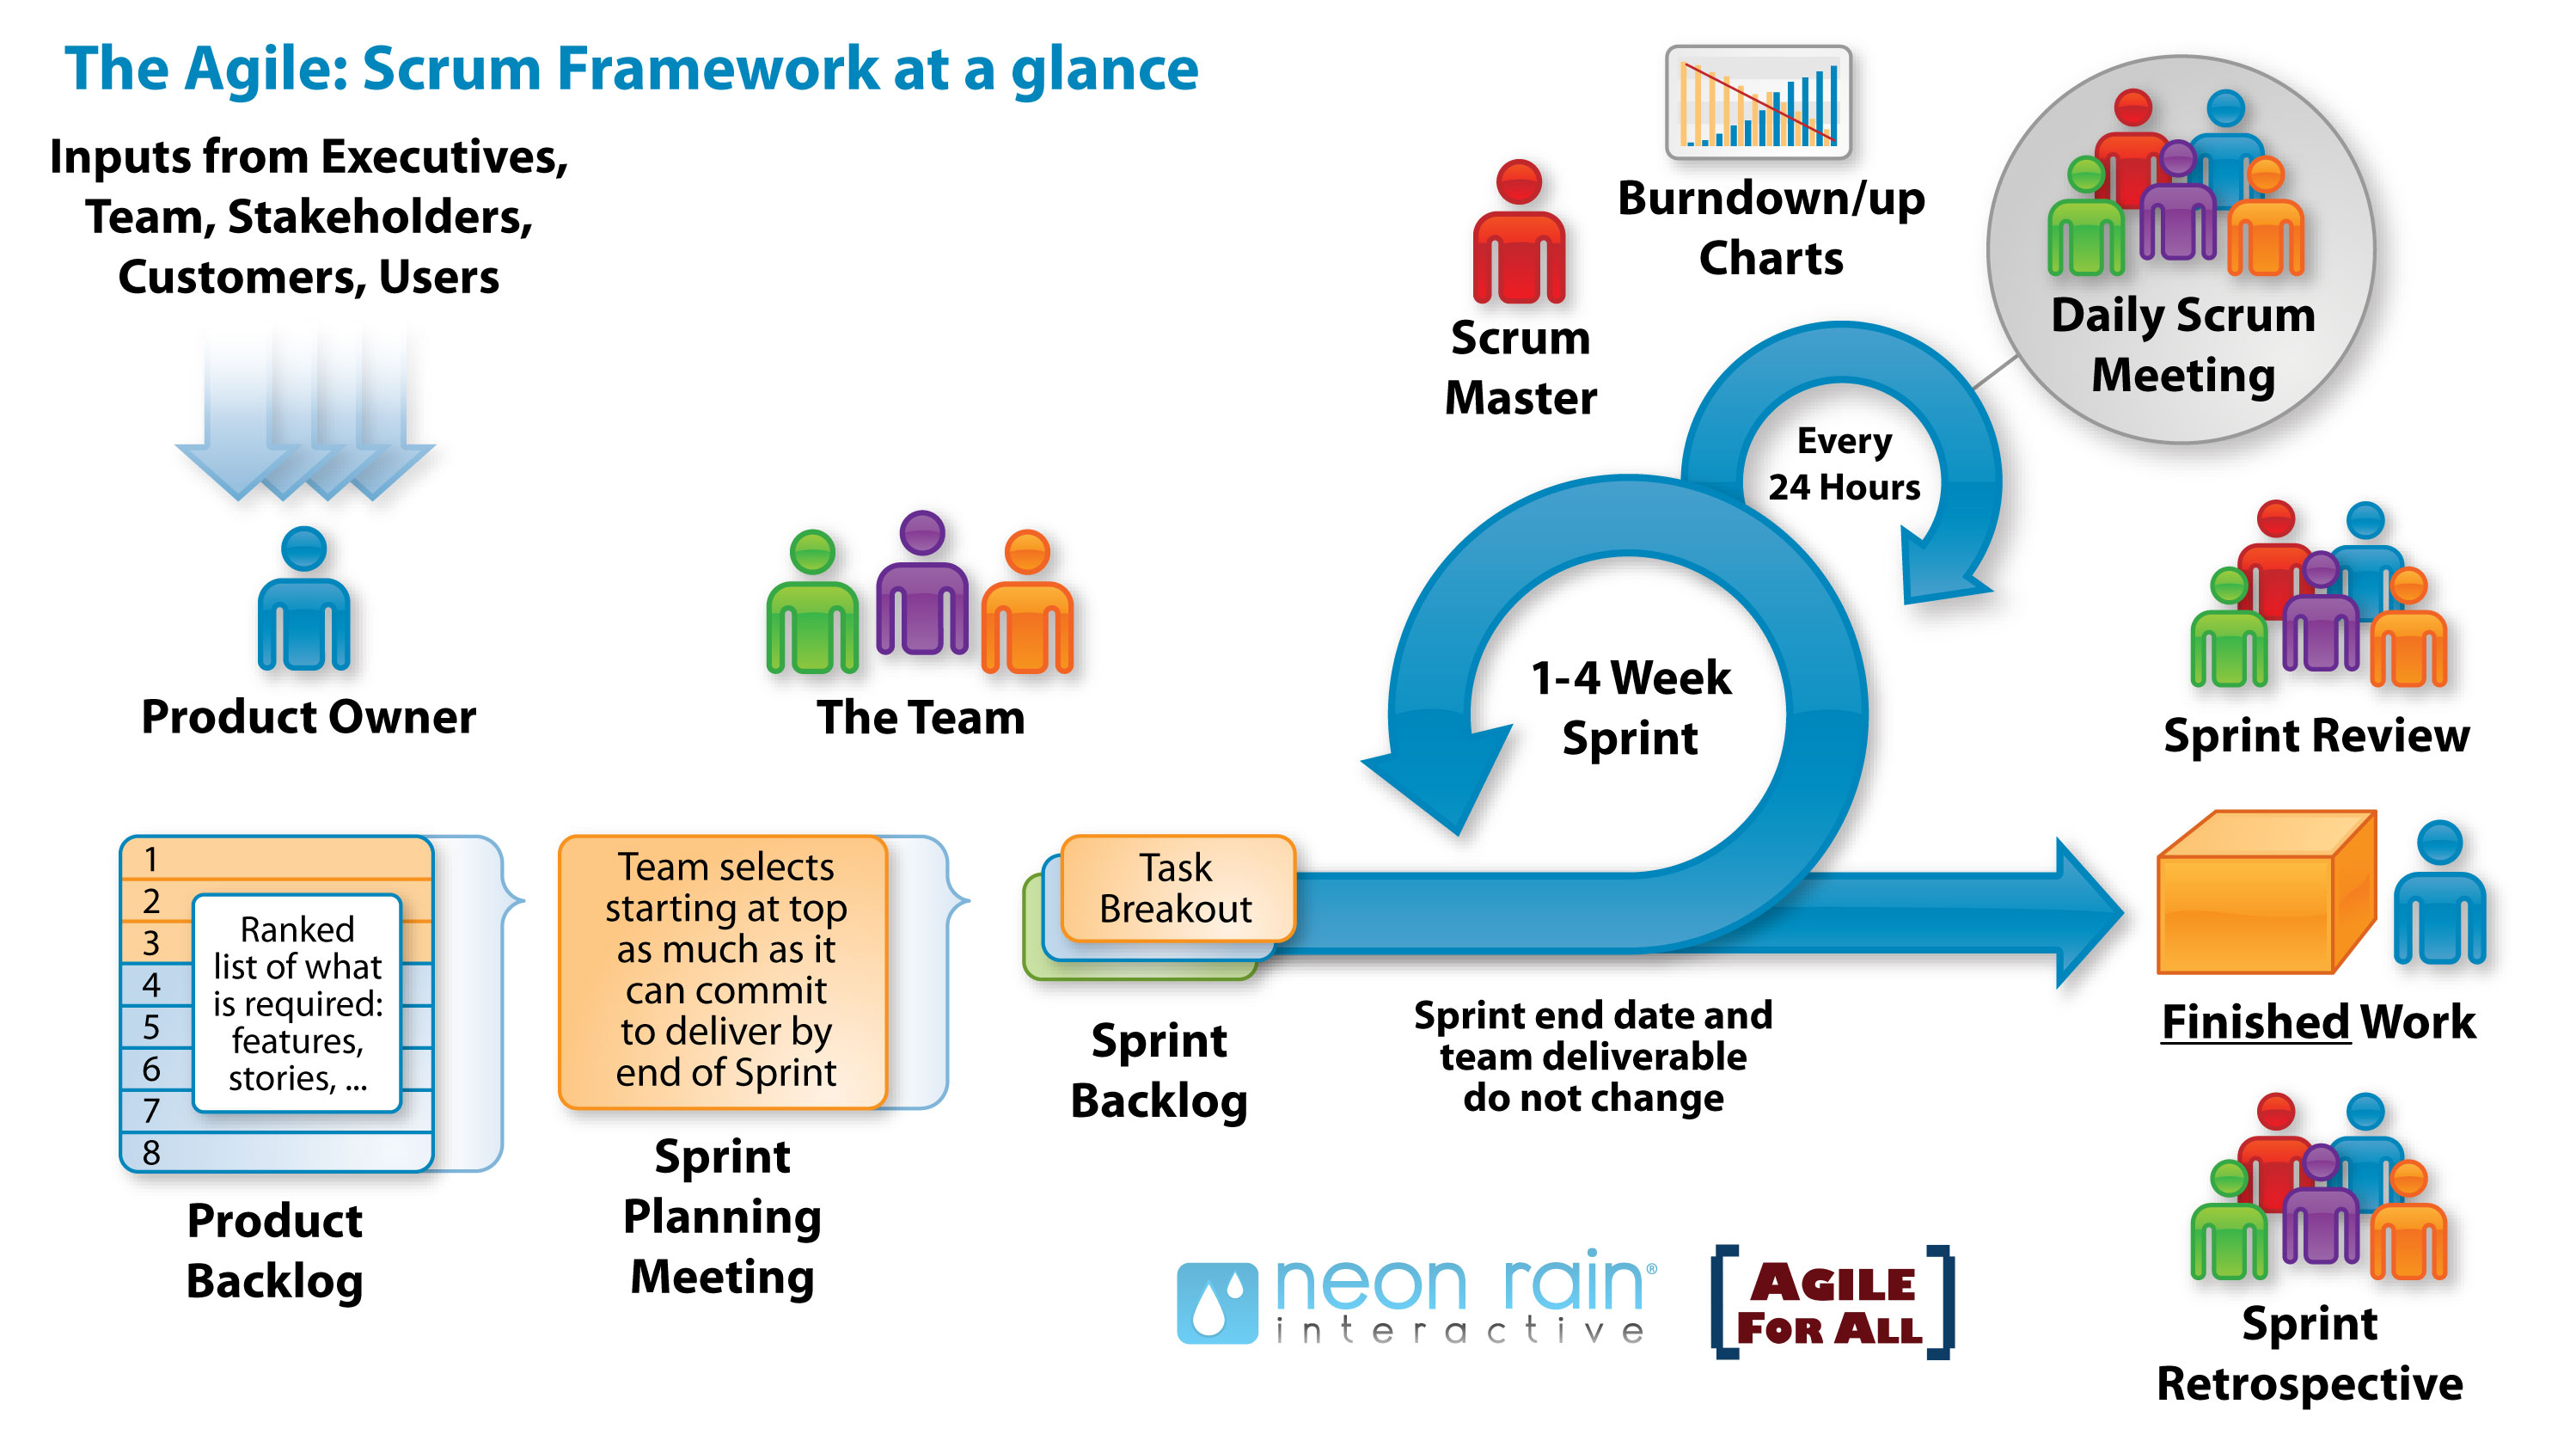
\includegraphics[width = \textwidth]{figs/Scrum.jpg}
  \end{figure}
\end{frame}

\begin{frame}
 \frametitle{Scrum - Adaptação Projeto}
  \begin{figure}
   \centering
   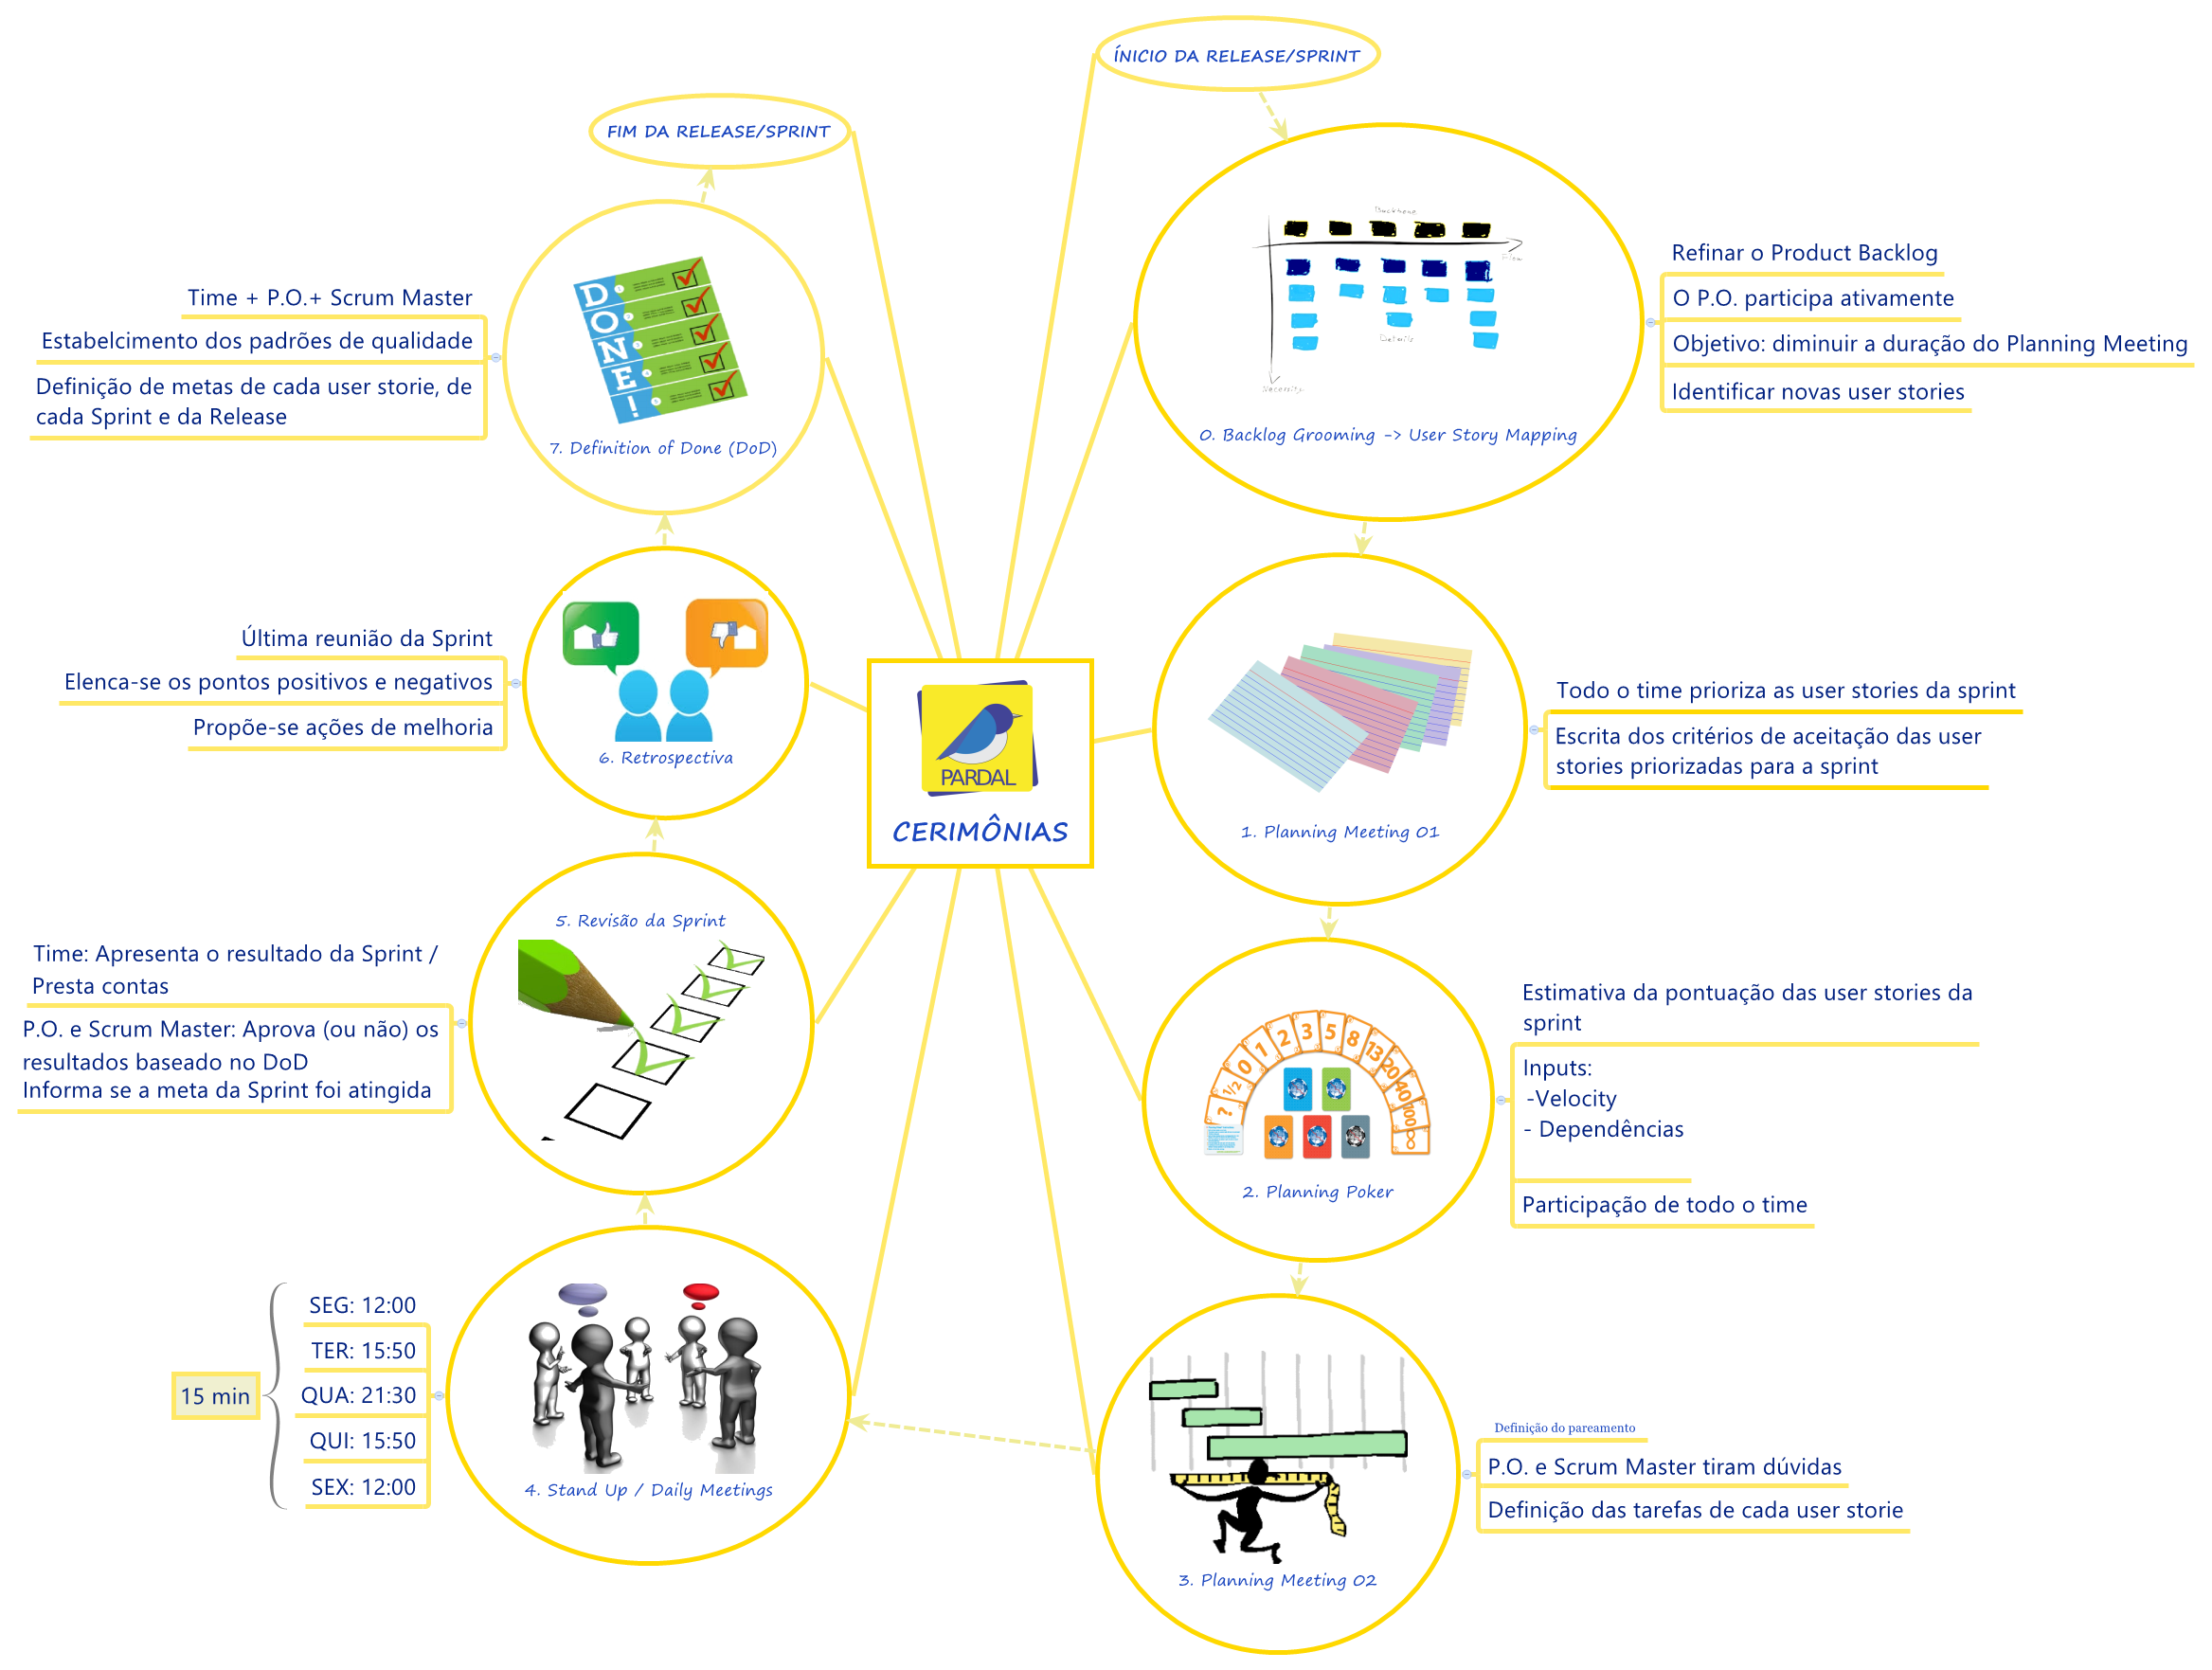
\includegraphics[width = \textwidth]{figs/Cerimonia.png}
  \end{figure}
\end{frame}

\begin{frame}
 \frametitle{Metodologia Ágil em Projetos}
  \begin{block}{}
 Maior parte dos projetos de software, o Scrum é aplicado com outras metodologias focadas na qualidade do produto (XP) e no fluxo contínuo de trabalho (Kanban)
 \end{block}

   \begin{figure}
   \centering
   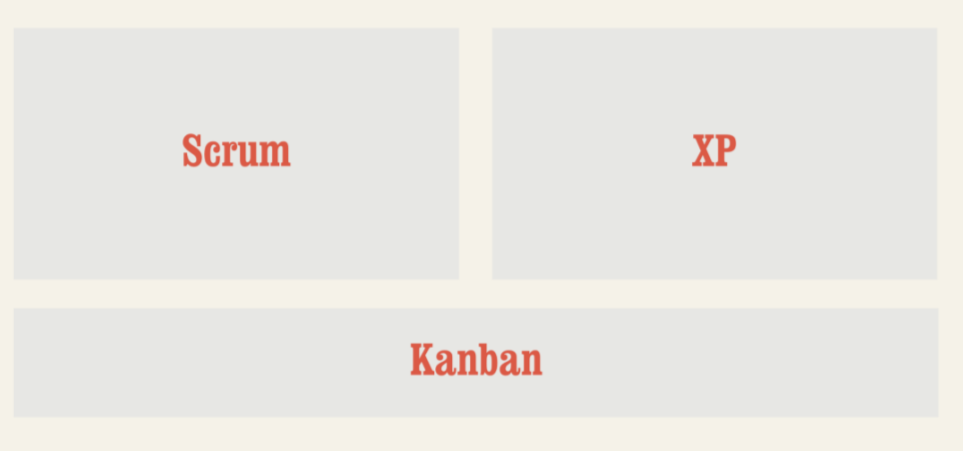
\includegraphics[width = 0.7\textwidth]{figs/cobertura_agil.png}
  \end{figure}
\end{frame}

\section{XP}
\begin{frame}
 \frametitle{eXtreming Programming}
 \begin{block}{}
  O XP é um método de desenvolvimento de software leve.
  O objetivo principal do XP é levar ao extremo um conjunto de práticas que são ditas como boas na engenharia de software
 \end{block}
 \begin{block}{}
  Como no Scrum, o XP prescreve iterações, artefatos e eventos
 \end{block}
\end{frame}

\begin{frame}
 \frametitle{XP diz}
 \begin{itemize}
  \item Já que testar é bom, que todos testem o tempo todo;
  \item Já que revisão é bom, que se revise o tempo todo;
  \item Se projetar é bom, então refatorar o tempo todo;
  \item Se teste de integração é bom, então que se integre o tempo todo;
  \item Se simplicidade é bom, desenvolva uma solução não apenas que funcione, mas que seja a mais simples possível;
  \item Se iterações curtas é bom, então mantenha-as realmente curtas;
 \end{itemize}
\end{frame}

\begin{frame}	
 \frametitle{XP Framework}
  \begin{figure}
   \centering
   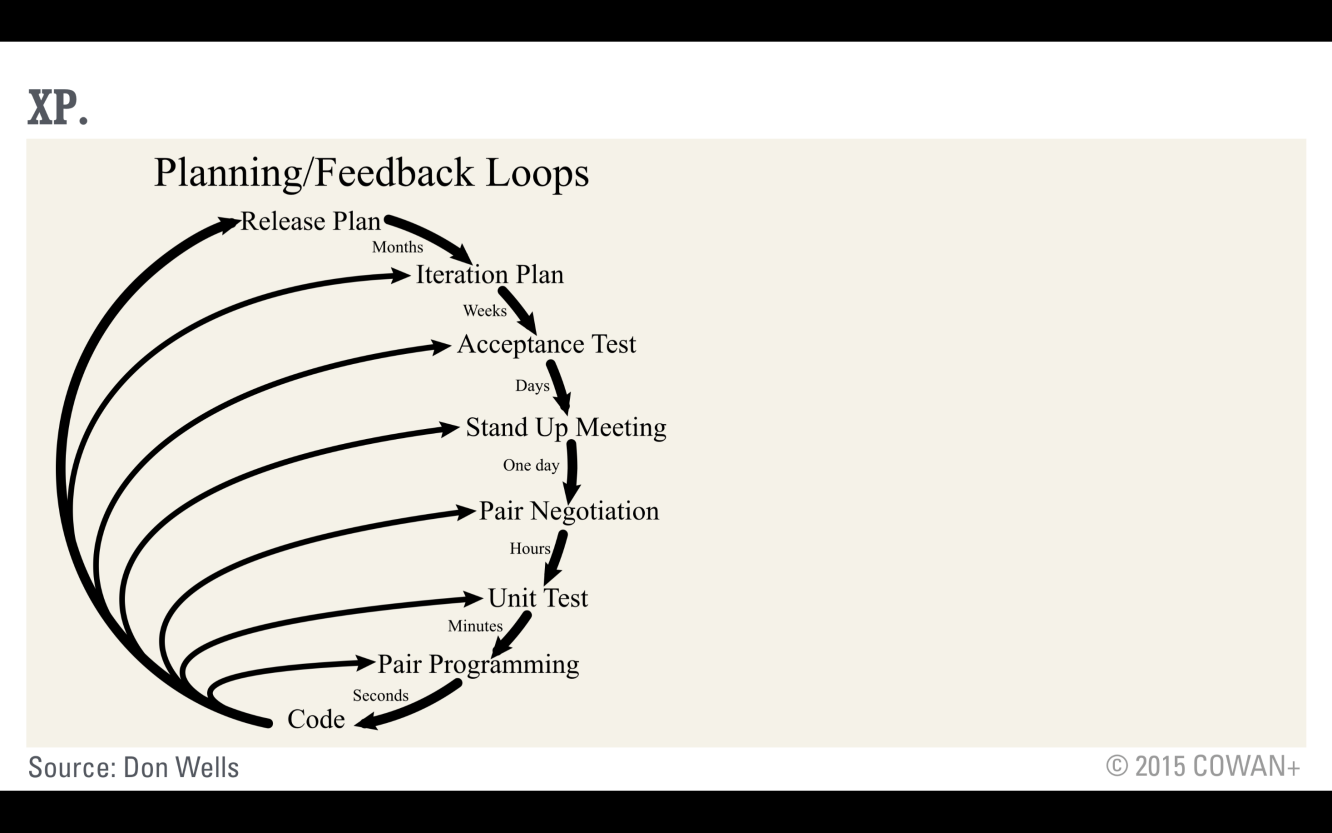
\includegraphics[width = \textwidth]{figs/xp_g.png}
  \end{figure}
\end{frame}

\begin{frame}
 \frametitle{XP - Funcionalidade "Pronta"}
 \begin{itemize}
  \item Uma funcionalidade "Pronta", significa:
  \begin{enumerate}
   \item Claramente codificada
   \item Refatorada
   \item Suite de testes automatizados (unitário, funcional, ...)
   \item Testes de aceitação
  \end{enumerate}
 \end{itemize}
\end{frame} 

\begin{frame}
 \frametitle{Atividades XP}
 \begin{itemize}
  \item  Listening - (escutar)
  \item  Testing - (testar)
  \item Coding - (codificar)
  \item Designing – (projetar)
 \end{itemize}
\end{frame}


\begin{frame}
 \frametitle{Práticas XP}
 \begin{itemize}
  \item Whole Team – Equipe
  \item Plannig Game – Jogo do planejamento
  \item Customer Tests – Testes de aceitação
  \item  Small releases – Versões pequenas
  \item  Simple Design – Projeto simples
  \item Pair programming – Programação em pares
  \item Test-driven Development – Desenvolvimento orientado a testes (TDD)
 \end{itemize}

\end{frame}

\begin{frame}
 \frametitle{Práticas XP}
 \begin{itemize}
  \item Refactoring – Refinamento do projeto
  \item Continuos Integration – Integração contínua
  \item Collective Ownership – Posse coletiva
  \item Coding Standards – Padrões de codificação
  \item Metaphor – Metáfora
  \item Sustainable Place – Ritmo saudável
 \end{itemize}
\end{frame}

\begin{frame}
 \frametitle{A equipe}
 \begin{itemize}
  \item  Todos em um projeto XP são parte de uma equipe.
  \item A equipe deve incluir um representante do cliente:
  \begin{itemize}
   \item estabelece os requisitos do projeto
   \item define as prioridades
   \item controla o rumo do projeto
  \end{itemize}
 \end{itemize}
\end{frame}

\begin{frame}
 \frametitle{A equipe}
 \begin{itemize}
  \item  Outros papéis assumidos pelos integrantes da equipe:
  \begin{itemize}
   \item programadores
   \item  testadores (que ajudam o cliente com testes de
aceitação)
    \item analistas (que ajudam o cliente a definir requerimentos)
    \item gerente (garante os recursos necessários)
    \item coach (orienta a equipe, controla a aplicação de XP)
    \item tracker (coleta métricas)
  \end{itemize}
 \end{itemize}
\end{frame}


\begin{frame}
 \frametitle{Jogo do Planejamento}
 \begin{itemize}
  \item Planejamento de um release
  \begin{itemize}
   \item  Cliente propõe funcionalidades desejadas (estórias)
    \item Programadores avaliam a dificuldade de
implementá-las
  \end{itemize}
  \item Planejamento de uma iteração
  \begin{itemize}
   \item Cliente define as funcionalidades prioritárias para a
iteração;
  \item Programadores as quebram em tarefas e avaliam o
seu custo (tempo de implementação)
  \end{itemize}
 \end{itemize}
\end{frame}

\begin{frame}
 \frametitle{XP - Teste Unitário}
 \begin{itemize}
  \item  Validar as classes básicas e os componentes do sistema 
  \item Verificar se o fluxo de controle e dados estão corretos
  \item  Realizado no início da iteração (TDD - Test driven development)
 \end{itemize}
\end{frame}

\begin{frame}
 \frametitle{XP - Relatando e Corrigindo Erros de Programação: 5 R's}
 \begin{itemize}
  \item \textbf{R}elatar um erro de programação
  \item \textbf{R}eproduzir o problema, ou então
  
  \textbf{R}eclassifica-lo como "não erro" (not a bug) ou "não será corrigido" (won't be fixed)
  \item criar um teste de \textbf{R}egressão que demonstre o erro
  \item \textbf{R}eparar o erro de programação
  \item \textbf{R}elançar o código reparado 
  
 \end{itemize}
\end{frame}

\begin{frame}
 \frametitle{XP - Programação Pareada}
 \begin{itemize}
  \item  Objetivo é a otimização da qualidade do software através  do desenvolvimento de um mesmo trecho de código por mais de uma pessoa
  \item Atividade cooperativa com duas funções diferentes: o piloto e observador
  \item Transferência de conhecimento entre a dupla
  \item Redução do tempo de desenvolvimento e melhoria da qualidade do software
 \end{itemize}
\end{frame}

\begin{frame}
 \frametitle{XP - Programação Pareada}
 \begin{itemize}
  \item Melhor qualidade do design, código e testes
  \item Revisão constante do código
  \item Nivelamento da equipe
  \item Maior comunicação
 \end{itemize}
\end{frame}

\begin{frame}	
 \frametitle{XP - Programação Pareada}
  \begin{figure}
   \centering
   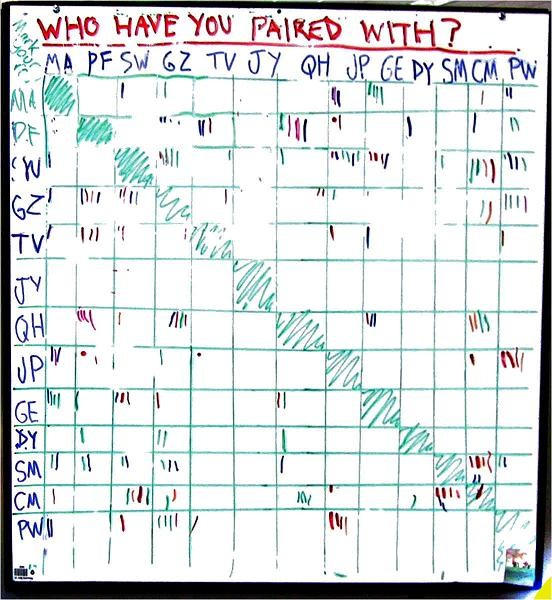
\includegraphics[width = \textwidth]{figs/pairing.png}
  \end{figure}
\end{frame}

\begin{frame}
 \frametitle{XP - Teste de Aceitação}
 \begin{itemize}
  \item  Teste de uma possível aceitação por parte do cliente
  \item Testes de aceitação estão intimamente ligados com as user stories
  \item  visam testar o sistema do ponto de vista do usuário
  \item Com testes de aceitação, voce sabe, sem dúvidas, quando o sistema está pronto.
 \end{itemize}
\end{frame}

\begin{frame}
 \frametitle{XP - Teste de Aceitação}
 \begin{itemize}
  \item  Originalmente chamado de teste de funcionalidade.
  \item São escritos pelo cliente. Este recebe o nome de cliente testador.
  \item São escritos no momento da escrita da user story.
  \item O cliente saberá como o sistema deve se comportar para que aquela user story seja considerada acabada.
  \item Para cada user story deve coexistir pelo menos 1 teste de aceitação.
  \item Uma user story só pode ser declarada terminada quando seus testes de aceitação executarem completamente.
 \end{itemize}
\end{frame}

\begin{frame}
 \frametitle{XP - Integração Contínua}
 \begin{itemize}
  \item o desenvolvedor integra o código alterado e/ou desenvolvido ao projeto principal na mesma frequência com que as funcionalidades são desenvolvidas, sendo feito muitas vezes ao dia ao invés de apenas uma vez
  \item o processo de build integrado deve ser feito constantemente, sendo sincronizado sempre que possível, evitando o acúmulo de códigos e de testes
 \end{itemize}
\end{frame}

\begin{frame}
 \frametitle{XP - Integração Contínua - Benefícios}
 \begin{itemize}
  \item Expõe o estado atual do desenvolvimento (viabiliza lançamentos pequenos e freqüentes)
  \item Estimula design simples, tarefas curtas, agilidade
  \item Oferece feedback sobre todo o sistema
  \item Permite encontrar problemas de design rapidamente
 \end{itemize}
\end{frame}


\begin{frame}
 \frametitle{Valores XP}
 \begin{itemize}
  \item Comunicação 
  \item Simplicidade
  \item Feedback
  \item Coragem
 \end{itemize}
\end{frame}

\begin{frame}
 \frametitle{Variáveis XP}
 \begin{itemize}
  \item O XP considera quatro as variáveis que estão presentes no desenvolvimento de um projeto
  \begin{enumerate}
   \item Custo
   \item Tempo
   \item Escopo
     \item Qualidade
  \end{enumerate}
 \end{itemize}
\end{frame}

\begin{frame}
 \frametitle{Variáveis XP}
 \begin{itemize}
  \item O planejamento dentro do XP é feito sempre da mesma maneira: as “forças externas” (clientes e gerentes) escolhem o valor de três destas variáveis,
  \item e a equipe de desenvolvimento projeta o valor conseqüente da quarta variável.
 \end{itemize}
\end{frame}

\begin{frame}
 \frametitle{Variáveis XP}
 É muito difícil encontrar uma relação ideal entre o peso de cada variável
 \begin{itemize}
  \item \textbf{Custo}: com um orçamento muito apertado normalmente não se consegue contar com a equipe que se gostaria, e isto pode trazer problemas para a efetiva resolução do problema do cliente.
 \end{itemize}
\end{frame}

\begin{frame}
 \frametitle{Variáveis XP}
 É muito difícil encontrar uma relação ideal entre o peso de cada variável
 \begin{itemize}
  \item \textbf{Escopo}:  um escopo menor pode melhorar a qualidade, pois se tem menos tarefas para serem desenvolvidas, além de reduzir o prazo e o custo
 \end{itemize}
\end{frame}

\begin{frame}
 \frametitle{Variáveis XP}
 É muito difícil encontrar uma relação ideal entre o peso de cada variável
 \begin{itemize}
  \item \textbf{Tempo}:  um prazo maior para a entrega final do sistema pode aumentar a qualidade e o escopo do mesmo, dentro de um limite. Por outro lado, caso o prazo seja muito pequeno, prejudica-se o escopo da aplicação.
 \end{itemize}
\end{frame}

\begin{frame}
 \frametitle{Variáveis XP}
 É muito difícil encontrar uma relação ideal entre o peso de cada variável
 \begin{itemize}
  \item \textbf{Qualidade}:  Pode-se ter ganhos pequenos (dias ou semanas) sacrificando a qualidade em alguns pontos do projeto, como por exemplo definindo-se um número menor de testes unitário para uma classe, a fim de poupar tempo de programação.
 \end{itemize}
\end{frame}

\begin{frame}
 \frametitle{Práticas XP}
  \begin{figure}
   \centering
   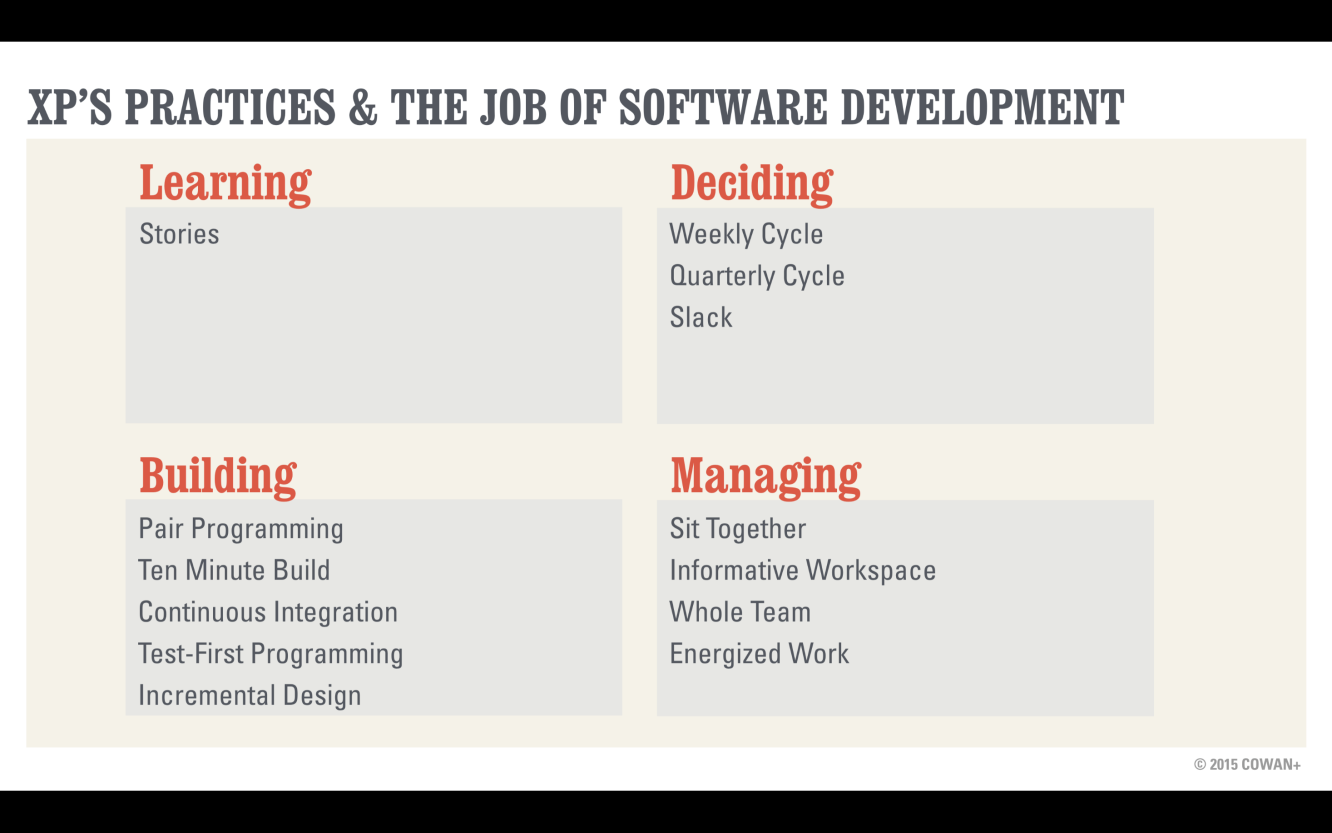
\includegraphics[width = \textwidth]{figs/xp_etapas.png}
  \end{figure}
\end{frame}

\begin{frame}
 \frametitle{Mantra Programador XP}
 \begin{itemize}
  \item Escute, para que saibamos qual é o problema a resolver e assim sendo conversar bastante com o cliente.
  \item Planeje, para que sempre que possamos fazer a coisa mais importante ainda a fazer. Planejamento é uma constante onde planejamos o tempo todo, incorporando no plano os toques de realidade que temos atualmente.
 \end{itemize}
\end{frame}

\begin{frame}
 \frametitle{Mantra Programador XP}
 \begin{itemize}
\item Codifique, senão o software não sai. XP é contra a documentação que não agrega valor, portanto enquanto um documento não é codificado ele é apenas um documento, dessa forma o documento mais importante é realmente o código.
\item Teste, senão não iremos realmente saber se está funcionando.
\item Refatore, senão o código vai ficar tão ruim que será impossível dar manutenção. Mantemos o espaço de trabalho sempre limpo através das práticas de refatoração.
 \end{itemize}

\end{frame}

\section{Work Flow - Kanban}
\begin{frame}
 \frametitle{Kanban}
  \begin{itemize}
  \item É um método para a implantação de mudanças que não prescreve papéis ou práticas específicas
  \item Oferece uma série de princípios que buscam melhorar o desempenho e reduzir desperdício, eliminando atividades que não agregam valor para a equipe.
  \item E um dos métodos de desenvolvimento de software menos prescritivo, se tornando adaptável a quase qualquer tipo de cultura.
 \end{itemize}
\end{frame}

\begin{frame}
 \frametitle{Kanban}
  \begin{itemize}
  \item Modelo visual do fluxo de trabalho da equipe, fica possível identificar o que realmente está sendo feito.
  \item O trabalho se torna visível, gerando uma serie de benefícios como, foco no “todo”, transparência e identificação de desperdícios
  \item Todos podem enxergar o contexto do outro, levando instantaneamente o aumento da comunicação e colaboração
 \end{itemize}
\end{frame}


\begin{frame}
 \frametitle{Kanban}
  \begin{figure}
   \centering
   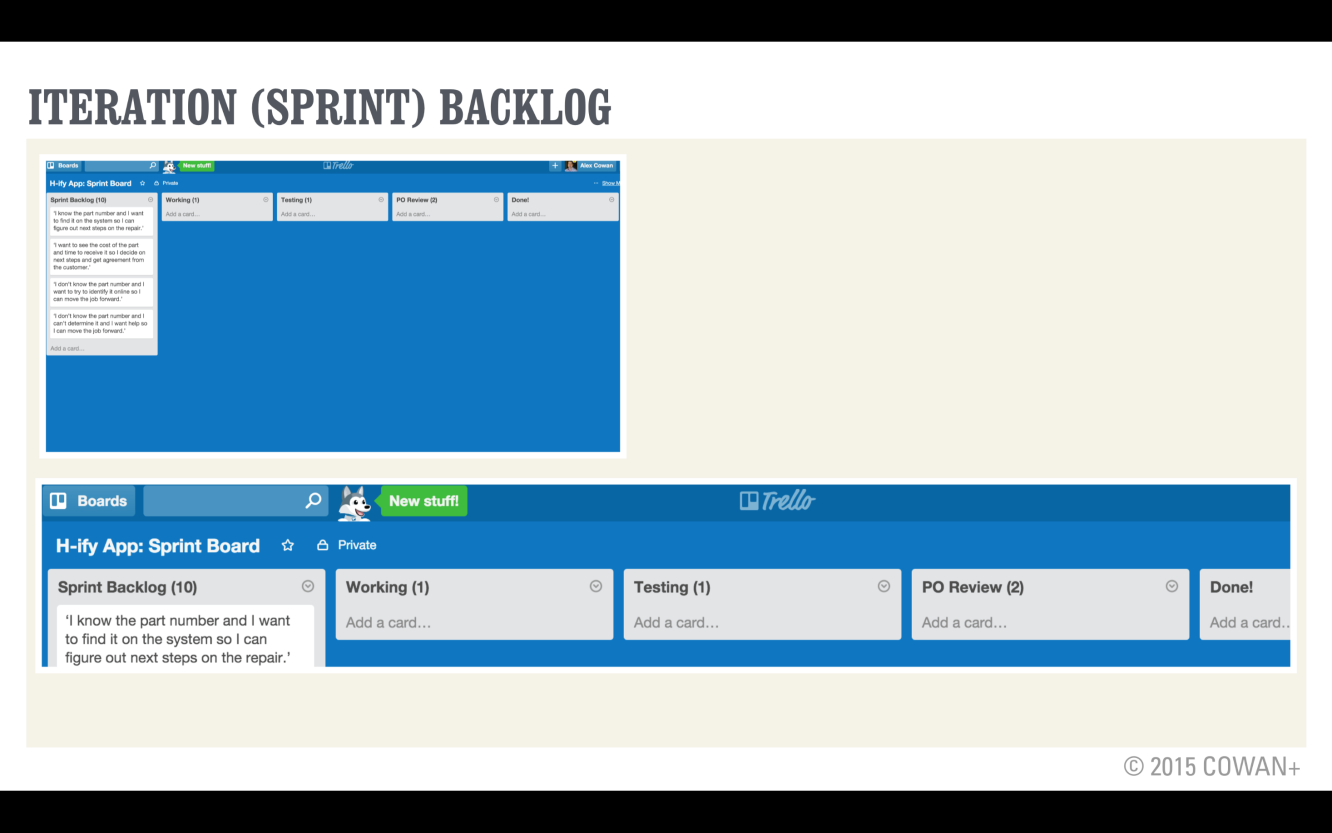
\includegraphics[width = \textwidth]{figs/kanban1.png}
  \end{figure}
\end{frame}

\begin{frame}
 \frametitle{Principios - Kanban}
  \begin{figure}
   \centering
   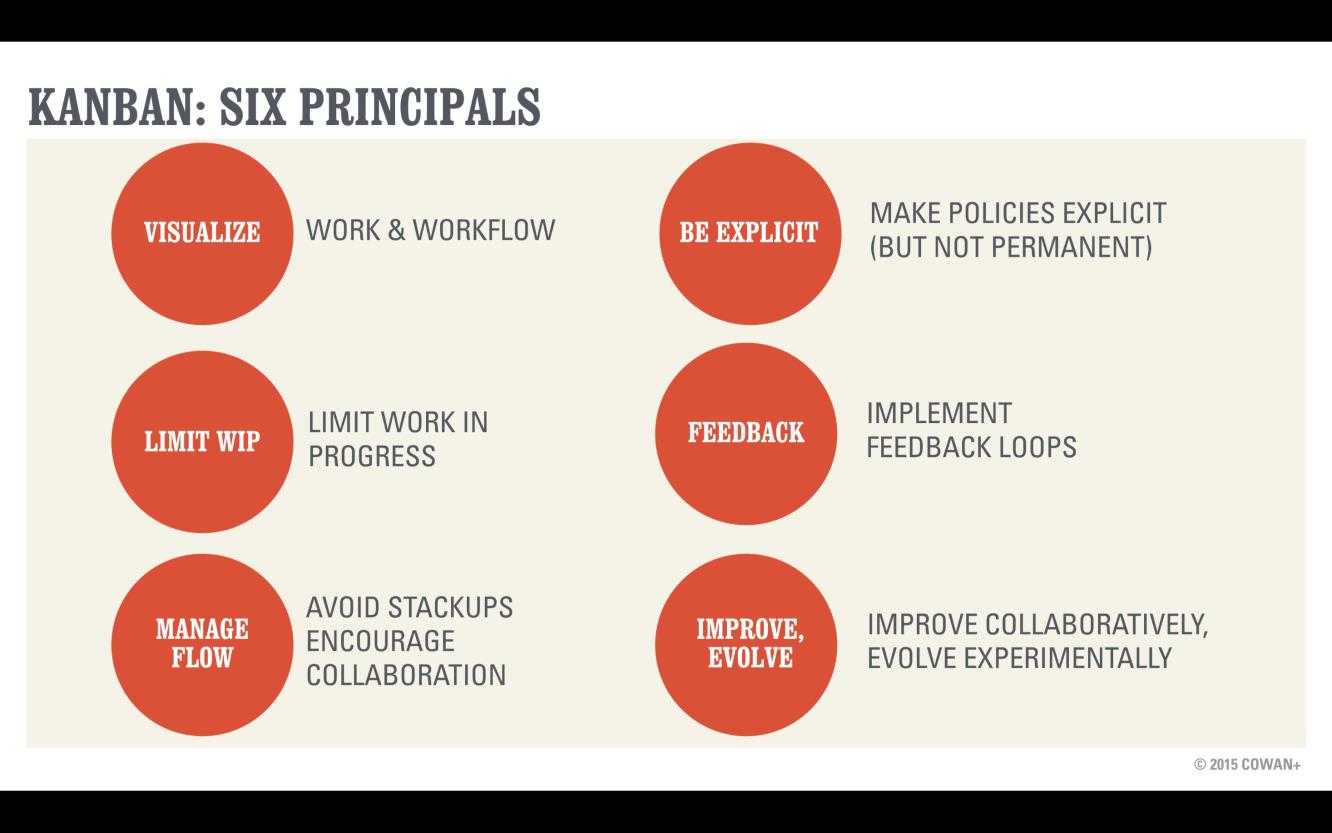
\includegraphics[width = \textwidth]{figs/kanban_principios.png}
  \end{figure}
\end{frame}

\begin{frame}
 \frametitle{Kanban - Work flow}
  \begin{figure}
   \centering
   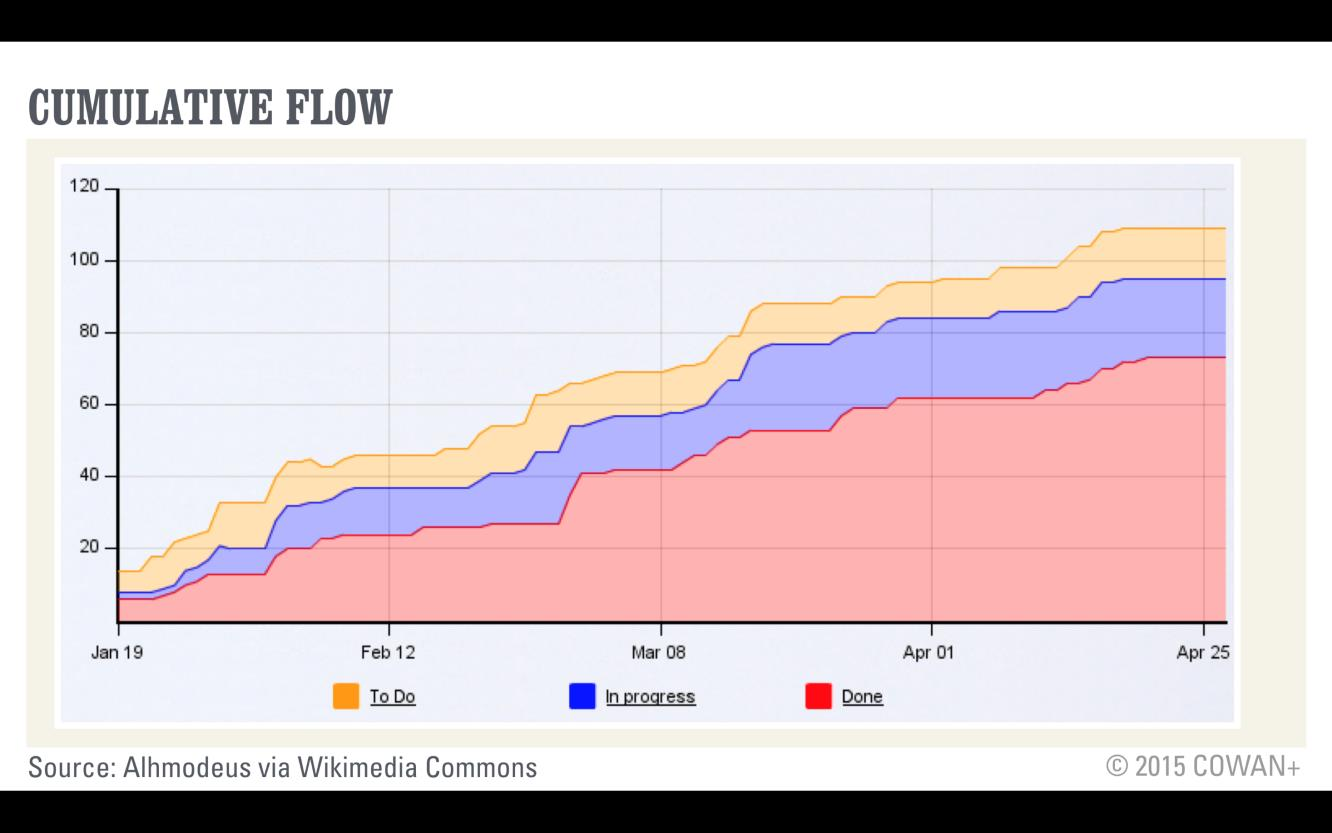
\includegraphics[width = \textwidth]{figs/workflow.png}
  \end{figure}
\end{frame}

\begin{frame}
 \frametitle{Kanban}
  \begin{itemize}
  \item Limitar a quantidade de trabalho em andamento (WIP)
  \item Gerenciar e medir o fluxo
  \item Tornar as políticas do processo explícitas
  \item Usar modelos para reconhecer oportunidades de melhoria
 \end{itemize}
\end{frame}

\begin{frame}
 \frametitle{Kanban - Classificação de itens e hierarquia}
  \begin{itemize}
  \item Épicos (Epics)
  \item Estória de usuário (User Story)
  \item Tarefas (Tasks)Tarefas (Tasks)
 \end{itemize}
\end{frame}

\begin{frame}
 \frametitle{Kanban - Evidenciando um quadro Kanban}
  \begin{figure}
   \centering
   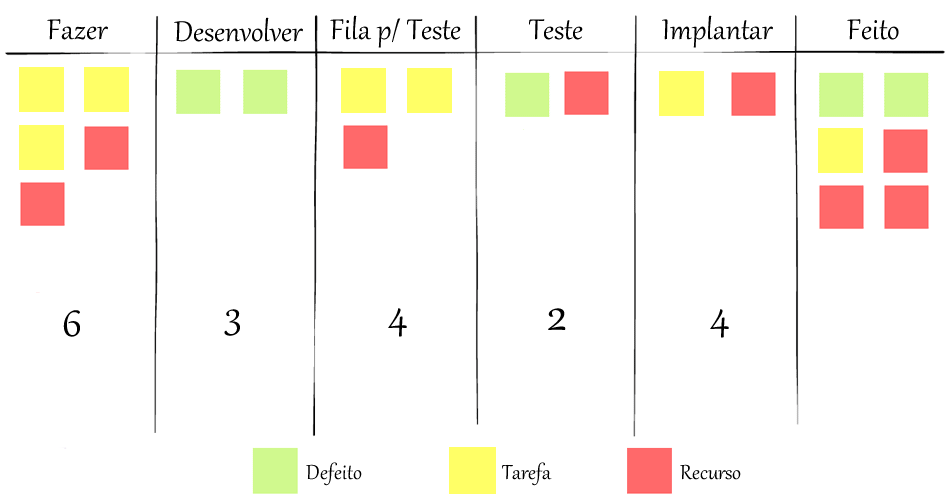
\includegraphics[width = \textwidth]{figs/kanban-quadro.png}
  \end{figure}
\end{frame}

\begin{frame}
 \frametitle{Kanban - Evidenciando um quadro Kanban}
  \begin{figure}
   \centering
   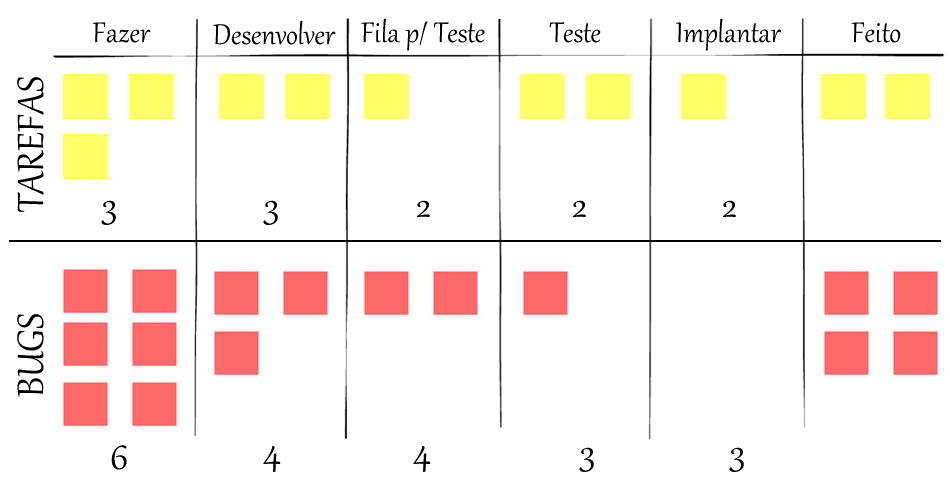
\includegraphics[width = \textwidth]{figs/kanban-quadro-rais.png}
  \end{figure}
\end{frame}

\begin{frame}
 \frametitle{Kanban - Beneficios}
  \begin{itemize}
  \item Tempo de ciclo curtos, oferecendo recursos mais rapidamente;
    \item Melhor gestão nas mudanças de prioridade;
    \item Requer menos organização;
    \item O processo é simplificado;
    \item Maior visibilidade dos projetos;
    \item Redução de desperdício;
    \item Redução de custo;
    \item Elimina atividades que não agregam valor para a equipe;
    \item Melhora a motivação e desempenho da equipe.
 \end{itemize}
\end{frame}

\section{Diferenças  Scrum, XP, Kanban}
\begin{frame}
 \frametitle{Diferenças  Scrum, XP, Kanban}
  \begin{figure}
   \centering
   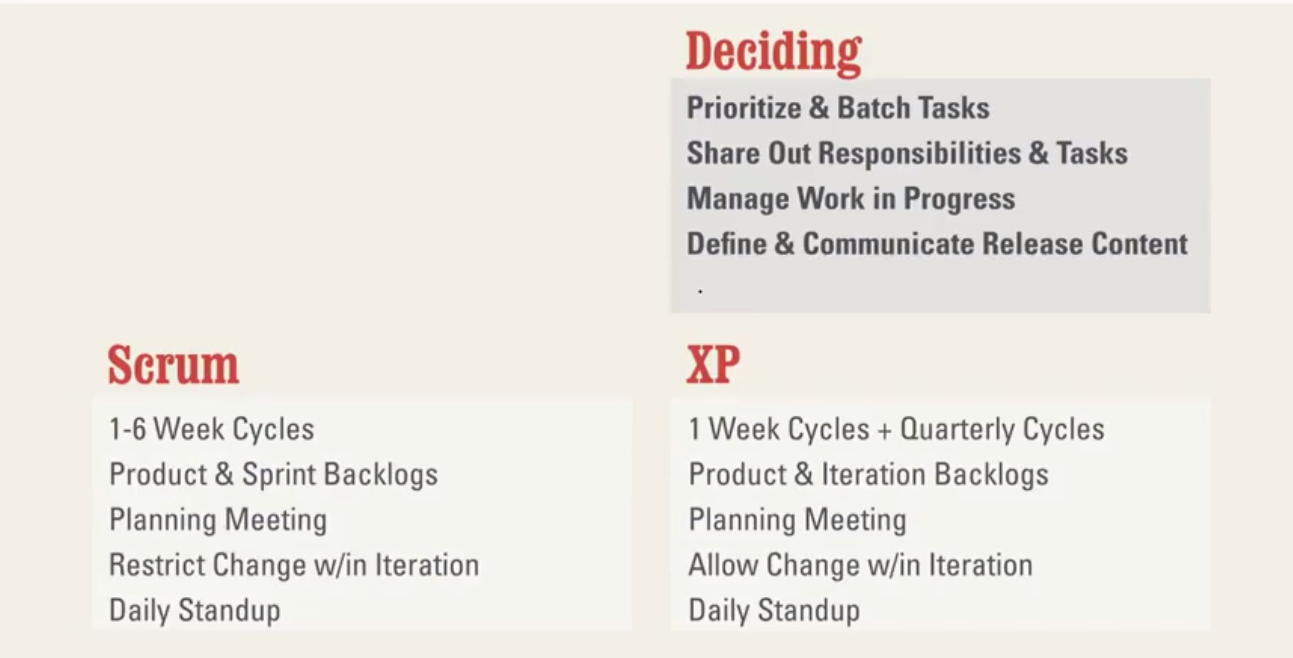
\includegraphics[width = \textwidth]{figs/deciding_scrum_xp.png}
  \end{figure}
\end{frame}



\section{Planejamento}
\begin{frame}
  \frametitle{Planejamento}
    \begin{itemize}
     \item Evento: Planning Meeting
     \item Artefato: Histórias de Usuário
     \item Estimativas: Velocity + Pontos/história
     \item Técnicas: planning game
     \item Transparência: kanban atualizado + Backlogs atualizados
    \end{itemize}
\end{frame}

\begin{frame}
  \frametitle{Planeje a iteração}
    \begin{itemize}
     \item Divida o projeto em iterações de 1 ou 2 semanas cada
     \item Escolha um dia da semana para fazer entregas
     \item Planeje reuniões periódicas e frequentes ( o ideal é o “standup meeting”)
     \item As iterações se tornam uma unidade de referência para o uso de métricas
     \item Entre no jogo para entregar software a cada iteração!
    \end{itemize}
\end{frame}



\begin{frame}
 \frametitle{Histórias de Usuários - Visão do sistema}
 \begin{block}{}
  Entendimento coletivo
  
Identificação clara dos objetivos a serem alcançados com o projeto
 \end{block}
 
  \begin{block}{}
 \begin{itemize}
  \item Como posso fazer direito algo que não não consigo explicar em poucas palavras?
  \item Como posso planejar uma jornada se não sei para onde seguir?
 \end{itemize}

 \end{block}
\end{frame}

\begin{frame}
 \frametitle{História de usuário}
 \begin{block}{}
  História de usuários deve poder ser testadas, ser pequenas o suficiente para que possam ser implementadas em uma iteração e deve possuir valor de negócio
 \end{block}
\end{frame}


\begin{frame}
 \frametitle{Histórias de usuário - Estrutura}
 \begin{enumerate}
     \item \textbf{Feature} [nome]
   \item    \textbf{Como um } [ tipo de stakeholder ]
   \item    \textbf{Para que} [ possa atingir algum objetivo ],
   \item    \textbf{Desejo} [ fazer alguma tarefa ]
 \end{enumerate}
\end{frame}


\begin{frame}	
 \frametitle{Histórias de usuário - Exemplo}
  \begin{figure}
   \centering
   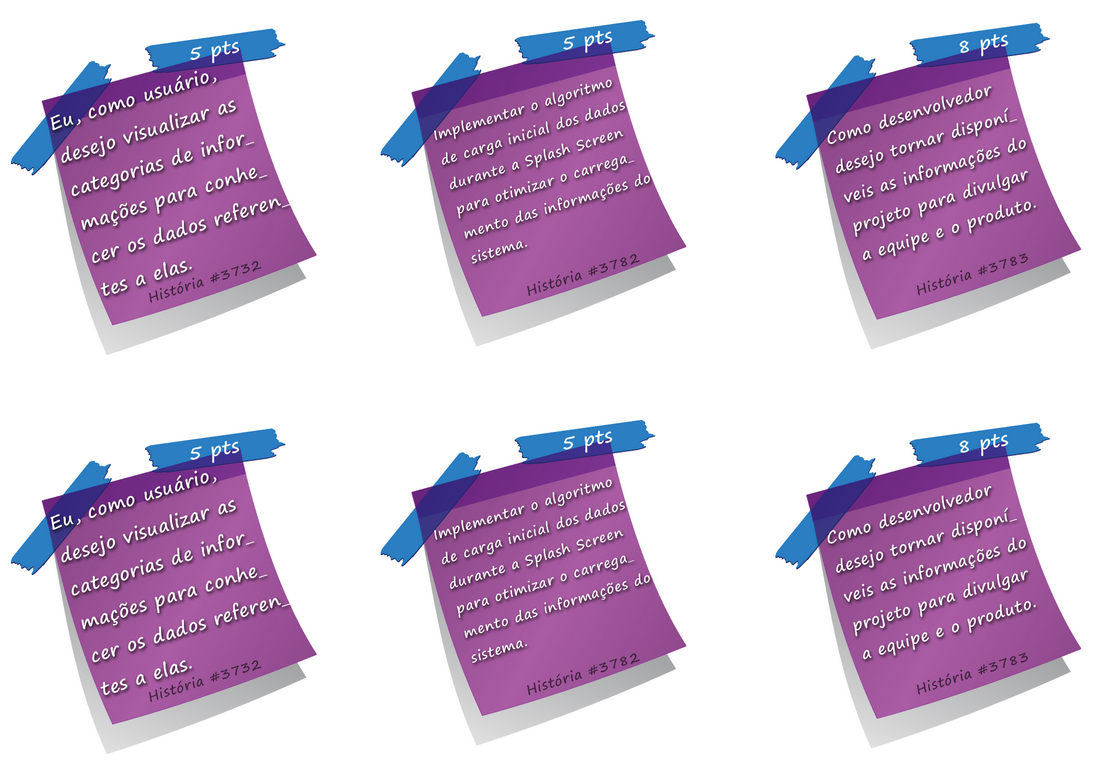
\includegraphics[width = \textwidth]{figs/fig7.png}
  \end{figure}
\end{frame}


\begin{frame}
 \frametitle{Histórias de usuário - O que faz uma boa história de usuário?}
 \begin{itemize}
  \item Acrônimo SMART oferece diretrizes concretas: 
  \begin{itemize}
   \item \textit{Specific} - Específico
   \item \textit{Measurement} - Mensurável
   \item \textit{Achievable} - Realizável
   \item \textit{Relevant} - Relevante
   \item \textit{Timeboxed} - Prazo fixo
  \end{itemize}
 \end{itemize}
\end{frame}

\begin{frame}
 \frametitle{Histórias de usuário - O que faz uma boa história de usuário?}
 \begin{itemize}
 \item Específico -  Devem ter pouco detalhe (digamos até 2 sentenças).
  \item Estimável - (entre 1 e 3 semanas).
  \item Mensurável - Testável (usando testes de aceitação)
  \item Relevante -São descritas pelo cliente.
  \item Prazo fixo - As estimativas de tempos são usadas para o planejamento de releases
  \item Não se limitam a descrever o que aparece na interface do usuário.
  \item Pelo menos 1 teste de aceitação automatizado deve existir para verificar que uma User Story foi implementada corretamente.
 \end{itemize}
\end{frame}


\begin{frame}
 \frametitle{Estimativas}
 \begin{itemize}
  \item \textbf{Ponto}: classificação de cada história de usuário, de acordo com sua complexidade de implementação
  \item \textbf{Velocidade}: a média de \textbf{pontos} por iteração que um grupo completa
 \end{itemize}
\end{frame}

\begin{frame}
 \frametitle{Velocidade}
 \begin{itemize}
  \item Velocidade está relacionada com a capacidade produtiva da equipe. Está relacionada a quantidade VS. tempo de Story Points que a equipe faz por iteração
  \item O Story Point corresponde ao esforço relacionado ao dia de trabalho ideal de um desenvolvedor
 \end{itemize}
\end{frame}

\begin{frame}
 \frametitle{Fator de Carga}
 \begin{itemize}
  \item O Fator de carga é relação entre o número de horas ideais e o número de horas disponíveis na iteração 
  \item Geralmente é calculado pela divisão do número de Story Points estimados vs. número de Story Points realizados na iteração. Ex: 14 SP / 9 SP = 1.55.
  \item Sempre que um desenvolvedor estimar o esforço de uma User Story, multiplique pelo fator de carga.
 \end{itemize}
\end{frame}

\begin{frame}
 \frametitle{Planning game}
 \begin{itemize}
  \item Essa prática é fundamental para elaborar a estratégia das interações, que é a forma como se trabalha o "cronograma" de um projeto com XP
  \item  basicamente define-se um tempo padrão para as interações e especifica-se quais e quantas estórias podem ser implementadas em uma interação
  \item O Planning Poker é uma prática de estimativa de tarefas bem simples e inclusive divertida
 \end{itemize}
\end{frame}

\begin{frame}
 \frametitle{Planning poker}
 \begin{itemize}
  \item Essa prática é fundamental para elaborar a estratégia das interações, que é a forma como se trabalha o "cronograma" de um projeto com XP
  \item  basicamente define-se um tempo padrão para as interações e especifica-se quais e quantas estórias podem ser implementadas em uma interação
  \item Considera, principalmente: Opinião  e Analogia
 \end{itemize}
\end{frame}

\begin{frame}
 \frametitle{Planning poker}
  \begin{figure}
   \centering
   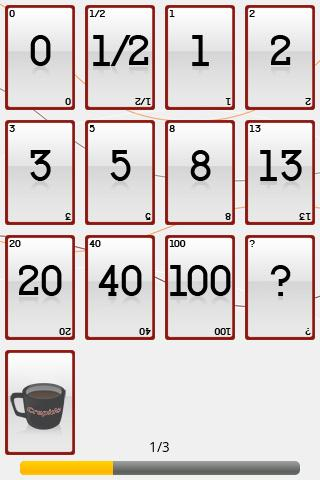
\includegraphics[height = \textheight]{figs/1352540079_screen.jpg}
  \end{figure}
\end{frame}

\begin{frame}
 \frametitle{Planning poker}
  \begin{figure}
   \centering
   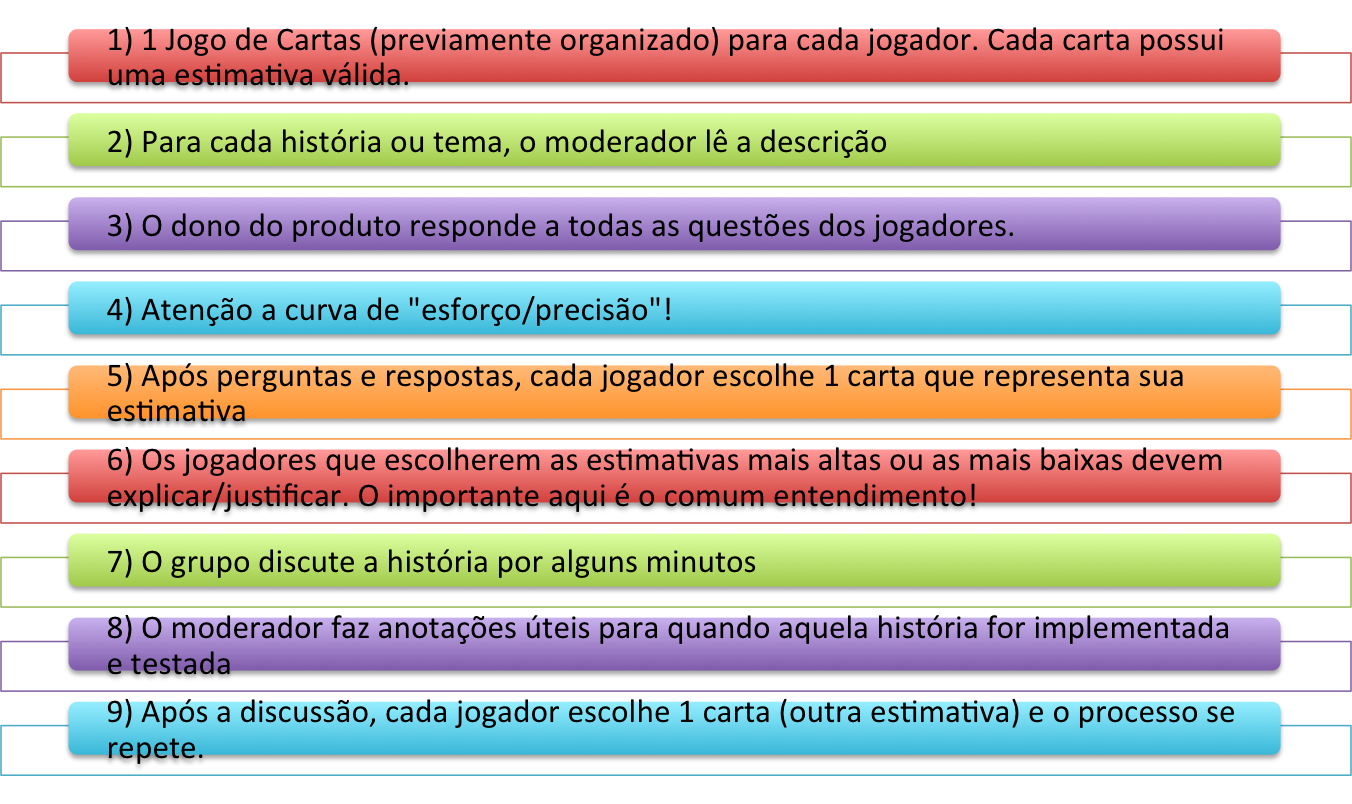
\includegraphics[width = 0.9\textwidth]{figs/planning_poker_aglo.png}
  \end{figure}
\end{frame}

\begin{frame}
 \frametitle{Planning poker - Objetivo}
  \begin{figure}
   \centering
   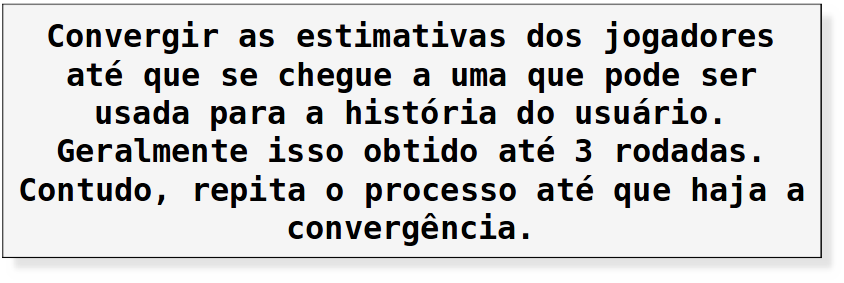
\includegraphics[width = 0.9\textwidth]{figs/obj_planning_poker.png}
  \end{figure}
\end{frame}	

\section{Projeto Guiado por Comportamento}
\begin{frame}
 \frametitle{Projeto guiado por comportamento - Método Agil}
 \begin{block}{}
  Projeto guiado por comportamento é o Desenvolvimento guiado por testes feito corretamente
 \end{block}
\end{frame}

\begin{frame}
 \begin{block}{Gerenciamento de Projeto: Scrum}
  Programação pareada e Sistemas de Controle de versão: "Não há vencedores em uma equipe perdedora,
  nem perdedores em uma equipe vencedora" (Fred Brooks)
 \end{block}
 \end{frame}
 
\begin{frame}
 \frametitle{Iteração do ciclo de vida de um programa Agil}
  \begin{figure}
   \centering
   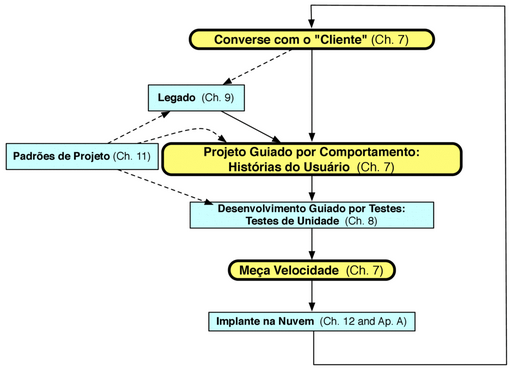
\includegraphics[width = 0.9\textwidth]{figs/fig1.png}
  \end{figure}
\end{frame}


\begin{frame}
 \frametitle{Ciclo de vida Agil}
 \begin{itemize}
  \item Trabalhar de maneira próxima e contínua com os \textit{stakeholders} para desenvolver requisitos e testes
  \item Manutenção do protótipo funcional enquanto novos produtos são implantados
  \item O desenvolvimento ágil não troca de fases
  \item O modo manutenção é presente desde o início da implementação
 \end{itemize}
\end{frame}

\begin{frame}
 \frametitle{Projeto Guiado por Comportamento (BDD)}
 \begin{itemize}
  \item O BDD (\textit{behavior Driven Development}) inicia o ciclo de vida ágil
  \item O BDD faz questionamento sobre o comportamento  de uma aplicação \textit{antes e durante o desenvolvimento}
  \item Os requisitos são continuamente aprimorados para assegurar que o software desenvolvido esteja de acordo com a vontade 	dos interessados
  \item O objetivo dos requisitos do BDD é \textbf{validação} (construir a coisa certa), não apenas \textbf{verificação} (fazer certo a coisa)
 \end{itemize}
\end{frame}

\begin{frame}
 \frametitle{Projeto Guiado por Comportamento (BDD)}
 \begin{itemize}
  \item Em BDD, a versão do conceito de requisitos são histórias de usuários, que descrevem como se espera que a aplicação seja usada
  \item Histórias de usuário ajudam os \textit{stakeholders} a planejar e priorizar o desenvolvimento
  \item Ao se concentrar no \textit{comportamento} da aplicação ao invés de se concentrar em sua \textit{implementação},  fica mais fácil reduzir
  mal-entendidos entre \textit{stakeholders}
 \end{itemize}
\end{frame}


